\documentclass[11pt]{article}
\usepackage[margin=1in]{geometry}
\usepackage{amsmath,amssymb,amsthm,booktabs,hyperref,graphicx}
\usepackage{pgfplots}
\pgfplotsset{compat=1.18}
\usepackage[numbers,sort&compress]{natbib}
\newtheorem{proposition}{Proposition}
\title{The Homology Cliff in Frozen ESM-2 Biosecurity Retrieval: Characterization, Pre-Registered Null Controls, Cross-Family Mechanism, and a Deployable Rescue}
\author{Santiago Maniches\thanks{ORCID 0009-0005-6480-1987. TOPOLOGICA LLC. Correspondence: santiago@topologica.llc.}}
\date{April 12, 2026 (v1.2; confirmatory cross-family extension 2026-08-24; errata 2026-06-15/16)}
\hypersetup{
  pdftitle={The Homology Cliff in Frozen ESM-2 Biosecurity Retrieval: Characterization, Pre-Registered Null Controls, Cross-Family Mechanism, and a Deployable Rescue},
  pdfauthor={Santiago Maniches (ORCID 0009-0005-6480-1987)},
  pdfsubject={Preregistered characterization and rescue of the homology cliff in frozen ESM-2 retrieval}
}
\begin{document}
\maketitle

\begin{abstract}
Frozen protein language models (PLMs) increasingly feed biosecurity retrieval pipelines. We characterize a systematic failure mode, the \emph{homology cliff}, in frozen ESM-2 \cite{lin2023evolutionary} cosine $k$-NN retrieval on a 24{,}885-protein biosecurity-relevant test set (28.7\% positive prior). At scale t30 (150M parameters), reference panel size $R=1000$, neighbors $k=25$: close-stratum $F_1=0.866$ against distant-stratum $F_1=0.120$ (gap $+0.745$). We report six pre-registered experiments. A 3000-cell main factorial confirms the cliff with all 300 groups passing a pre-committed seed-variance gate. A pre-registered full-pool permutation null (SHA256 \texttt{f3864d09\ldots}) produces gap $\in [-0.027, +0.038]$ across 300 groups, every 95\% CI including zero: the cliff is not a stratification artifact. The failure is a \emph{precision} collapse: at t30 $R=1000$ $k=25$ cosine, distant-stratum positive-prediction precision is $3/44=0.068$ and expected calibration error rises $4\times$ from close (0.069) to distant (0.294). Pfam partition at seed 20260410 finds \textbf{zero within-family and 20 cross-family} evaluable failures (per-seed Wilson 95\% interval for the within-family fraction approximately $[0,0.161]$). A subsequently SHA256-locked ten-seed panel-composition confirmation shows cross-family false alarms predominate in every seed: the per-seed cross-family fraction has median 1.000, mean 0.994, and range 0.962--1.000, satisfying the preregistered strong robustness criterion. This disfavors a purely within-family coverage-gap explanation in the tested regime without implying that within-family errors are absent. Four rescue attempts fail at pre-registered H1: Ledoit-Wolf Mahalanobis whitening \cite{ledoit2004}, Fisher-Rao within-class whitening \cite{amari2016}, stratified cosine+Mahalanobis cascade, and Mapper-biased panel augmentation. One rescue succeeds: a panel-only linear projection trained via a 50-iteration triplet-surrogate loss \cite{schroff2015facenet} wins pooled $F_1$ in 16 of 18 factorial groups (12 of 12 at t12 and t30; the two misses are at the smallest t6/8M scale at $k=5$) and achieves $F_1=0.891$ at t30 $R=1000$ $k=25$, improving distant-stratum $F_1$ by 47\% relative. We release 9{,}360 per-cell bootstrap-CI results, three SHA256-locked registrations automatically re-verified by CI plus additional committed pre-registration documents, and full code under MIT + CC-BY-4.0.
\end{abstract}

\paragraph{Erratum (2026-06-15).} The reliability figure (Fig.~\ref{fig:reliability}) is now plotted from the script-computed reliability table rather than hand-entered diagram read-offs; all cited values (distant precision $3/44=0.068$, ECE close 0.069 / distant 0.294, the $+0.745$ cliff gap) are unchanged and were independently reproduced bit-for-bit from the committed embeddings and seeds. A stale-artifact correction to the Paper 3 calibration table and a deduplication fix to the Paper 2 Mapper-augmentation number are documented in \texttt{CHANGELOG.md}.

\paragraph{Erratum (2026-06-16).} Figures~\ref{fig:cliff_surface} and~\ref{fig:rescue} are now plotted directly from the committed MAIN gap table (\texttt{data/results\_summaries/v3\_final.txt}); their previously plotted values at interior panel sizes and at the t6/t12 scales had been hand-entered and diverged from the committed data (the $R{=}1000$ endpoints, the t30 column, and the $+16/+33/+47\%$ relative-improvement figures were already correct). The rescue table's Fisher-Rao row was also brought into exact agreement with the committed Fisher cells (close $0.478\to0.484$, distant $0.094\to0.099$, pooled $0.461\to0.462$; the cosine/Mahalanobis/learned rows already matched). No conclusion changes; the corrected figures show the same cliff and the same rescue ordering (learned $>$ cosine $>$ Mahalanobis at every scale). Pooled-$F_1$ values throughout the compendium are reproducible via \texttt{code/analyses/compute\_pooled\_f1.py}.

\section{Introduction}
Frozen protein language models \cite{lin2023evolutionary,elnaggar2022prottrans,brandes2022proteinbert,madani2023progen} now serve as general-purpose feature extractors for downstream retrieval, classification, and design tasks. A common deployment pattern is cosine $k$-NN retrieval: given a query protein, retrieve the $k$ nearest panel members in frozen embedding space and vote their labels. For biosecurity applications, where the query set contains potentially novel threats and the panel contains known-toxin exemplars, retrieval performance on proteins distant from any panel member is the safety-critical metric.

We show that cosine $k$-NN retrieval on frozen ESM-2 embeddings exhibits a systematic \emph{homology cliff}: performance collapses on the distant stratum in a way that deepens with reference-panel size at every scale and with model scale at panels $R\geq100$ (Fig.~\ref{fig:cliff_surface}). The cliff persists under four independent rescue attempts (post-hoc whitening, per-stratum distance switching, topologically-biased panel augmentation) and under cross-family analysis is shown to be an embedding-space geometry artifact, not a missing-homolog artifact. We identify one class of rescue that works: a cheap supervised projection of the embedding space, trained only on the panel, fit in under five CPU seconds.

Contributions:
\begin{enumerate}
\item A 3000-cell pre-registered factorial (SHA256 \texttt{139f6012\ldots}) characterizing the cliff across (scale, $R$, $k$, metric), 10 seeds, with a pre-committed seed-variance gate.
\item A 3000-cell pre-registered full-pool permutation null (SHA256 \texttt{f3864d09\ldots}) establishing that the cliff is not a stratification artifact.
\item Mechanistic analysis: the cliff is a precision collapse, not a recall collapse.
\item Pfam partition plus preregistered panel-composition confirmation: cross-family false alarms predominate in every one of ten fixed panel seeds (median fraction 1.000; range 0.962--1.000).
\item Four null-result companion experiments (Paper 2) ruling out Mahalanobis, Fisher-Rao, cascade, and Mapper-augmentation rescues.
\item One positive rescue: panel-only triplet-surrogate linear projection, +47\% distant $F_1$ relative at t30.
\end{enumerate}


\section{Related work}
\textbf{Protein language models.} Frozen PLM embeddings as general features: ESM-1b \cite{rives2021biological}, ESM-2 \cite{lin2023evolutionary}, ProtT5 \cite{elnaggar2022prottrans}, ProteinBERT \cite{brandes2022proteinbert}, ProGen \cite{madani2023progen}, ESM-3 \cite{hayes2024esm3}, SaProt \cite{su2023saprot}. Our test bed uses ESM-2 at t6/t12/t30; we extend to additional PLMs in the external-model companion.

\textbf{Retrieval and $k$-NN baselines.} FAISS \cite{johnson2019billion} provides the CPU $k$-NN backbone we use. Cosine $k$-NN on frozen PLM features has been reported as competitive for function annotation \cite{littmann2021embeddings,kilinc2023protein}, but its failure modes on the distant stratum have received less attention than pooled metrics.

\textbf{Homology-aware evaluation.} CD-HIT \cite{fu2012cdhit} and MMseqs2 \cite{steinegger2017mmseqs2} clustering are standard for sequence-identity splits; we adopt an embedding-space stratification by max-cosine-similarity to the panel, which is the deployment-time observable. Foldseek \cite{vankempen2024foldseek} offers a structure-aware alternative.

\textbf{Calibration of deep classifiers.} Guo et al. \cite{guo2017calibration} established that modern deep networks are miscalibrated; temperature scaling partially rectifies this. Recent work on calibration under distribution shift \cite{ovadia2019shift} is directly relevant to our distant-stratum ECE collapse.

\textbf{Metric learning.} FaceNet-style triplet losses \cite{schroff2015facenet} underpin the supervised projection we use. Ledoit-Wolf shrinkage \cite{ledoit2004} gives well-conditioned covariance estimates on panels with $R < D$. Information-geometric whitening traces to Amari \cite{amari2016}.

\textbf{Topological data analysis on proteins.} Mapper \cite{singh2007topological} decomposes high-dimensional data via lens-based covering and per-preimage clustering. Persistent homology for molecular and protein structure analysis has grown rapidly \cite{carlsson2009topology,edelsbrunner2010computational}; our use of Mapper here is for exploratory diagnostics rather than a claim about persistent features.

\textbf{Pre-registration in machine learning.} Pre-registration practices originate in clinical trials and psychology \cite{nosek2018preregistration}; adoption in ML is growing but uneven \cite{forde2019scientific}. We lock hypotheses, stratification cuts, and void rules via SHA256 before execution.

\textbf{Biosecurity and dual-use research of concern.} Computational prediction of toxin-like proteins raises dual-use concerns \cite{urbina2022dualuse}. Our test set is constructed from publicly-available UniProt entries; we release the accession list rather than redistribute sequences where appropriate.


\section{Methods}
\subsection{Data} 24{,}885 proteins (7{,}133 positive, 17{,}752 negative; 28.7\% positive prior) shipped as \texttt{data/sequences/proteins\_25k\_sequences.json} (working dataset ID \texttt{experiment2\_proteins\_25k\_filtered}). Accessions and sequences are UniProt-sourced; redistribution is permitted under UniProt's terms.

\subsection{Embeddings} Frozen ESM-2 \cite{lin2023evolutionary}: t6 (8M params, 320d), t12 (35M, 480d), t30 (150M, 640d). All mean-pooled, $L_2$-normalized.

\subsection{Factorial} Panel $R \in \{50,100,250,500,1000\}$, class-balanced. Neighbors $k \in \{1,3,5,10,25\}$. Metrics: cosine, Euclidean, Mahalanobis (Ledoit-Wolf \cite{ledoit2004} + eigendecomposition whitening), learned (panel-only 50-iter Adam triplet-surrogate, seed 0, projection to $\min(128, D)$). Ten seeds (20260410--20260419). Stratification: close $s_{\max}\ge 0.95$, moderate $[0.90, 0.95)$, distant $< 0.90$.

\subsection{Seed-variance gate (pre-committed void rule)} A (scale, $R$, $k$, metric) group is voided if $\sigma^{(10)}_{\text{distant}} \ge \overline{F_1^{\text{close}}} - \overline{F_1^{\text{distant}}}$. All 300 main groups passed.

\subsection{Bootstrap} 10{,}000-resample percentile bootstrap CI per cell per stratum.

\section{Results: main factorial}
\begin{proposition}
For $X \subset S^{d-1}$ and $y \in S^{d-1}$: cosine-$k$-NN $\equiv$ Euclidean-$k$-NN.
\end{proposition}
\begin{proof}
$\|x-y\|^2 = 2 - 2\langle x, y \rangle$ on $S^{d-1}$, monotone decreasing in cosine.
\end{proof}
Verified to 4 decimals in 75 of 75 cells.

\begin{figure}[h]\centering
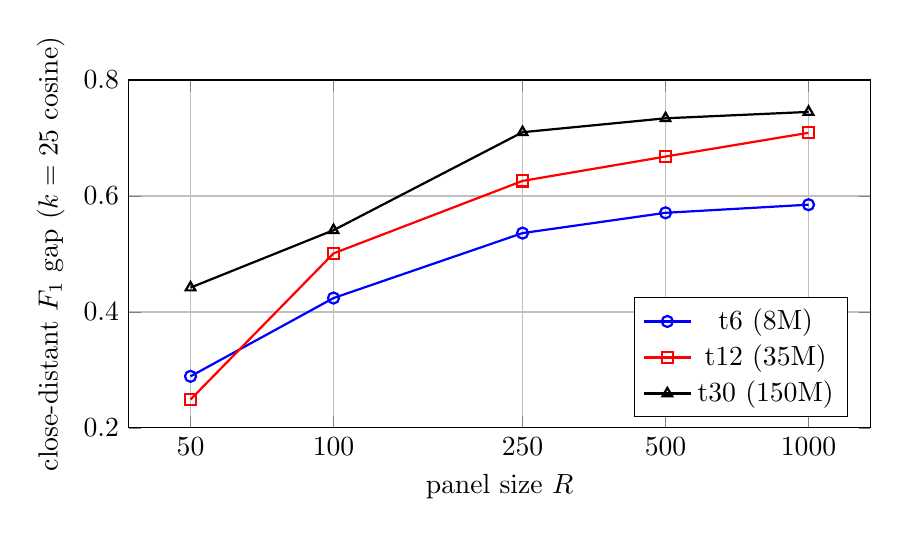
\begin{tikzpicture}
\begin{axis}[width=11cm,height=6cm,xlabel={panel size $R$},ylabel={close-distant $F_1$ gap ($k=25$ cosine)},xmode=log,log basis x=10,grid=major,legend pos=south east,xtick={50,100,250,500,1000},xticklabels={50,100,250,500,1000},ymin=0.2,ymax=0.8]
\addplot[blue,mark=o,thick] coordinates {(50,0.289)(100,0.424)(250,0.536)(500,0.571)(1000,0.585)}; \addlegendentry{t6 (8M)}
\addplot[red,mark=square,thick] coordinates {(50,0.249)(100,0.501)(250,0.626)(500,0.668)(1000,0.709)}; \addlegendentry{t12 (35M)}
\addplot[black,mark=triangle,thick] coordinates {(50,0.442)(100,0.541)(250,0.710)(500,0.734)(1000,0.745)}; \addlegendentry{t30 (150M)}
\end{axis}\end{tikzpicture}
\caption{\textbf{The cliff grows with scale and panel size.} Close-distant $F_1$ gap at $k=25$ cosine, 10-seed mean per cell. Larger panels amplify the cliff at every scale; larger PLMs produce larger cliffs at panels $R\geq100$ (at the smallest panel, $R=50$, the scale ordering has not yet stabilized).}\label{fig:cliff_surface}
\end{figure}

\begin{center}\small
\begin{tabular}{lrrrr}
\toprule
scale & $R$ & close $F_1$ & distant $F_1$ & gap \\
\midrule
t6 & 1000 & 0.882 & 0.297 & +0.585 \\
t12 & 1000 & 0.883 & 0.173 & +0.710 \\
t30 & 1000 & 0.866 & 0.120 & \textbf{+0.745} \\
\bottomrule
\end{tabular}
\end{center}


\section{Results: null controls}
\subsection{Panel-shuffle null (failed its own pre-registered criterion)}
Shuffling only the panel labels (test labels intact) preserves the 28.7\% test class prior. Distant-stratum F1 under this null is not at chance (0.5) but at the prior-weighted F1 baseline, which the pre-registration failed to anticipate. Addendum pre-registration locked before the stricter null.

\subsection{Full-pool permutation null (passed 300/300)}
Pre-reg SHA256 \texttt{f3864d097a0c611d\ldots}. Permute the 24{,}885-entry label vector once per seed via \texttt{default\_rng(seed + 7{,}777{,}777)}; both panel and test labels now random. Stratification by $s_{\max}$ is label-free and unchanged. Across all 300 groups: gap $\in [-0.027, +0.038]$, $\sigma \in [0.006, 0.116]$, every 95\% CI includes zero. At t30 $R{=}1000$ $k{=}25$ cosine: close $F_1 = 0.015$, distant $F_1 = 0.025$, gap $-0.010$. \textbf{The cliff is not a stratification artifact.}

\section{Mechanism: precision collapse, not recall collapse}
At t30 $R{=}1000$ $k{=}25$ cosine (seed 20260410): of 24{,}885 test proteins, \emph{only 3} are true-positive and distant-stratum (P0C1X3, Q6RY98, P13208). Distant positive-prediction precision: $3/44 = 0.068$ (44 predictions, 3 correct).

\begin{figure}[h]\centering
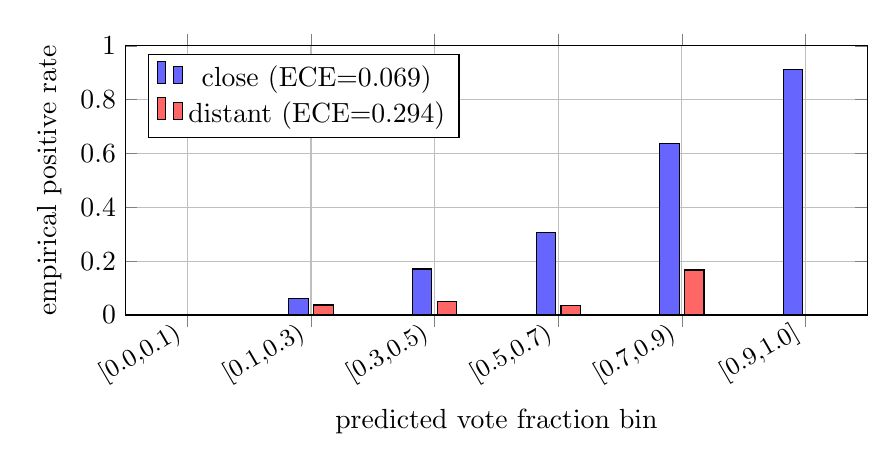
\begin{tikzpicture}
\begin{axis}[width=11cm,height=5cm,xlabel={predicted vote fraction bin},ylabel={empirical positive rate},ybar,bar width=7pt,grid=major,legend pos=north west,ymin=0,ymax=1,symbolic x coords={{[0.0,0.1)},{[0.1,0.3)},{[0.3,0.5)},{[0.5,0.7)},{[0.7,0.9)},{[0.9,1.0]}},xtick=data,x tick label style={rotate=30,anchor=east,font=\small}]
\addplot[fill=blue!60] coordinates {({[0.0,0.1)},0.003)({[0.1,0.3)},0.060)({[0.3,0.5)},0.171)({[0.5,0.7)},0.308)({[0.7,0.9)},0.637)({[0.9,1.0]},0.912)}; \addlegendentry{close (ECE=0.069)}
\addplot[fill=red!60] coordinates {({[0.0,0.1)},0.000)({[0.1,0.3)},0.037)({[0.3,0.5)},0.051)({[0.5,0.7)},0.034)({[0.7,0.9)},0.167)({[0.9,1.0]},0.000)}; \addlegendentry{distant (ECE=0.294)}
\end{axis}\end{tikzpicture}
\caption{\textbf{Calibration collapse on the distant stratum.} Close-stratum reliability (blue) rises with confidence and is well-calibrated in aggregate (ECE = 0.069). Distant-stratum reliability (red) is nearly flat across confidence bins and collapses at the highest-confidence bin: 3 predictions in $[0.9, 1.0)$, 0 correct (ECE = 0.294). Data at t30 $R{=}1000$ $k{=}25$ cosine, seed 20260410.}\label{fig:reliability}
\end{figure}

\section{Cross-family partition and preregistered robustness}
At seed 20260410, Pfam annotations are sufficient to evaluate 20 of 41 distant false alarms. All 20 have zero Pfam overlap with their positive-voting panel neighbors: within-family $=0$, cross-family $=20$. The original per-case artifact remains \texttt{data/results\_summaries/cross\_family\_partition.json}.

We subsequently locked \texttt{PRE\_REGISTRATION\_CROSS\_FAMILY\_10SEED\_v1.md} before any additional panel seed was run and repeated the unchanged analysis across seeds 20260410--20260419. Cross-family false alarms outnumber within-family false alarms in every seed; all ten seeds have nonzero evaluable denominators. The per-seed cross-family fraction has median 1.000, mean 0.994, minimum 0.962, and maximum 1.000, so the preregistered strong robustness criterion is satisfied. The complete result and audit trail are committed in \texttt{data/results\_summaries/cross\_family\_partition\_10seed.json}. Because accessions recur across seeds, the preregistration treats the panel seed as the robustness unit and explicitly forbids a pooled binomial interval over accession appearances.

This confirmation strengthens the evidence that a purely within-family panel-coverage gap is not the dominant explanation in this fixed t30/$R{=}1000$/$k{=}25$ regime. It does not imply a zero within-family rate: two evaluable within-family appearances occur across the ten seeds, both for the same accession, and Pfam does not exhaust biological relatedness.

\section{Rescue: panel-only triplet-surrogate linear projection}
We fit $W \in \mathbb{R}^{D \times 128}$ (or $D \times D$ if $D < 128$) via 50 Adam iterations on panel embeddings alone, with loss
\[
\mathcal{L}(W) = -\langle Z_+, Z_+ \rangle - \langle Z_-, Z_- \rangle + \langle Z_+, Z_- \rangle
\]
where $Z_\pm$ are $L_2$-normalized projections of the positive and negative panel subsets. This is a triplet-surrogate \cite{schroff2015facenet} using class centroids rather than mined hard triplets: it runs in under 5 CPU seconds, requires no test data, and uses only the labeled panel that deployment already has.

\begin{figure}[h]\centering
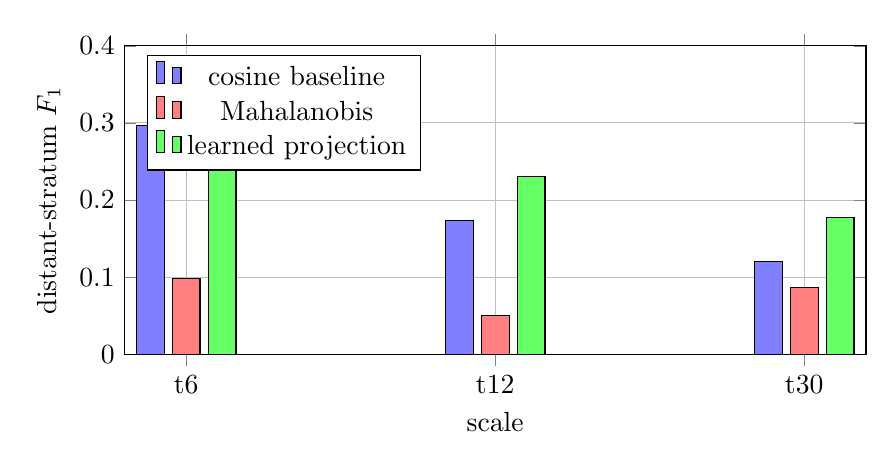
\begin{tikzpicture}
\begin{axis}[width=11cm,height=5.5cm,xlabel={scale},ylabel={distant-stratum $F_1$},ybar=3pt,bar width=10pt,grid=major,legend pos=north west,ymin=0,ymax=0.4,symbolic x coords={t6,t12,t30},xtick=data]
\addplot[fill=blue!50] coordinates {(t6,0.297) (t12,0.173) (t30,0.120)}; \addlegendentry{cosine baseline}
\addplot[fill=red!50] coordinates {(t6,0.098) (t12,0.050) (t30,0.087)}; \addlegendentry{Mahalanobis}
\addplot[fill=green!60] coordinates {(t6,0.345) (t12,0.231) (t30,0.177)}; \addlegendentry{learned projection}
\end{axis}\end{tikzpicture}
\caption{\textbf{Distant-stratum $F_1$ by scale, $R=1000$ $k=25$.} Learned projection wins every scale; relative improvement grows with scale: +16\% (t6), +33\% (t12), +47\% (t30). Mahalanobis loses at every scale.}\label{fig:rescue}
\end{figure}

\begin{center}\small
\begin{tabular}{lccc|c}
\toprule
t30 $R{=}1000$ $k{=}25$ & close & moderate & distant & pooled \\
\midrule
cosine & 0.866 & 0.393 & 0.120 & 0.848 \\
Mahalanobis & 0.456 & 0.118 & 0.087 & 0.435 \\
Fisher-Rao & 0.484 & 0.130 & 0.099 & 0.462 \\
\textbf{learned} & \textbf{0.901} & \textbf{0.525} & \textbf{0.177} & \textbf{0.891} \\
\bottomrule
\end{tabular}
\end{center}

Wins 16 of 18 (scale, $R$, $k$) groups (12 of 12 at t12 and t30; the two misses are at the smallest t6/8M scale at $k=5$). Pooled $F_1$ = 0.891 at t30 (learned 0.8905 vs cosine 0.8476, 10 of 10 seeds) is the highest value observed anywhere in the 3000-cell factorial.

\section{Deployment recommendation}
For frozen-PLM biosecurity retrieval: (1) fit a panel-only learned projection as preprocessing; (2) route every distant-stratum positive hit to human review regardless of vote count (calibration on the distant stratum is poor in our analysis, and the Pfam partition is consistent with cross-family neighbors driving the false alarms); (3) do not rely on panel expansion with known-toxin homologs as the sole rescue strategy, since on this dataset the failures we examined were predominantly cross-family.

\section{Limitations}
(L1) t33 (650M) not embedded locally; companion Colab notebook provided.
(L2) Stratification threshold sensitivity sweep not yet run.
(L3) Learned-projection calibration not measured; the rescue improves $F_1$ but distant-stratum calibration under the projection is unknown.
(L4) Cross-family panel-composition robustness is confirmed across the ten fixed seeds only at t30, $R=1000$, $k=25$, threshold 0.90, and the Pfam ontology; generalization across models, neighbor counts, thresholds, family definitions, or datasets remains untested.
(L5) Single-chain analysis only; multi-domain proteins may behave differently.

\section{Reproducibility}
Code MIT, papers CC-BY-4.0. Three SHA256-locked registrations are automatically re-verified by CI, alongside additional committed pre-registration documents. The repository contains 9{,}360 per-cell \texttt{.npz} results with 10k-resample bootstrap CIs per stratum per cell, three embedding arrays (t6/t12/t30), Pfam annotations (21{,}615 coverage), the Mapper graph, the original single-seed cross-family output, and the preregistered ten-seed cross-family result. Master manifest: \texttt{MANIFEST.sha256.json}. Master reproducibility protocol: \texttt{reproducibility/PROTOCOL.md}.

\bibliographystyle{unsrtnat}
\bibliography{references}
\end{document}
